\appendix
\section{Qualitative Results}\label{app:qualitative-results}
This section shows more qualitative results generated via an initial run of the code provided with the original hyperparameters as well. It is divided into results generated via correctly classified images, and results generated via incorrectly classified images.
\subsection{Correctly Classified Explanations}
\begin{figure}[H]
    \centering
    \includegraphics[width=0.7\textwidth]{images/qualitative_ims/correct_qualitative_ims/goldfish_gradcam.png}
    \caption{Qualitative results using the goldfish example image.}
    \label{fig:app-goldfish}
\end{figure}
\begin{figure}[H]
    \centering
    \includegraphics[width=0.7\textwidth]{images/qualitative_ims/correct_qualitative_ims/bluejay_gradcam.png}
    \caption{Qualitative results using the jay example image.}
    \label{fig:app-jay}
\end{figure}
\begin{figure}[H]
    \centering
    \includegraphics[width=0.7\textwidth]{images/qualitative_ims/correct_qualitative_ims/chikadee_gradcam.png}
    \caption{Qualitative results using the chickadee example image.}
    \label{fig:app-chickadee}
\end{figure}
\subsection{Incorrectly Classified Images}


\begin{figure}[H]
    \centering
    \includegraphics[width=0.7\textwidth]{images/qualitative_ims/incorrect_qualitative/gas_mask.png}
    \caption{Qualitative results using the terrier example image.}
    \label{fig:app:terrier}
\end{figure}
\begin{figure}[H]
    \centering
    \includegraphics[width=0.7\textwidth]{images/qualitative_ims/incorrect_qualitative/sea_slug.png}
    \caption{Qualitative results using the lionfish example image.}
    \label{fig:app-lionfish}
\end{figure}
\begin{figure}[H]
    \centering
    \includegraphics[width=0.7\textwidth]{images/qualitative_ims/incorrect_qualitative/snail.png}
    \caption{Qualitative results using the bottlecap example image.}
    \label{fig:app-bottlecap}

\end{figure}

\begin{figure}[H]
    \centering
    \includegraphics[width=0.7\textwidth]{images/qualitative_ims/incorrect_qualitative/spider_web.png}
    \caption{Qualitative results using the lizard example image.}
    \label{fig:app-lizard}

\end{figure}

\subsection{Additional VGG-16 Images}


\begin{figure}[H]
    \centering
    \includegraphics[width=0.7\textwidth]{images/qualitative_ims/vgg_qualitative/birds_vgg_grad.png}
    \caption{PixelRDE and CartoonX outputs when using the VGG16 model.}
    \label{fig:app-birds-vgg}

\end{figure}

\subsection{Obfuscation Distribution Scaling Example Images}

\begin{figure}[H]
    \centering
    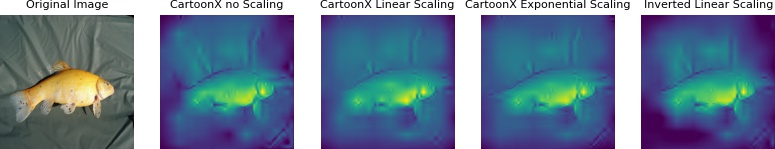
\includegraphics[width=0.7\textwidth]{images/qualitative_ims/obfuscation_examples/tench.JPEG}
    \caption{Obfuscation experimentation qualitative results for the image of a tench.}
    \label{fig:app-tench}

\end{figure}
\begin{figure}[H]
    \centering
    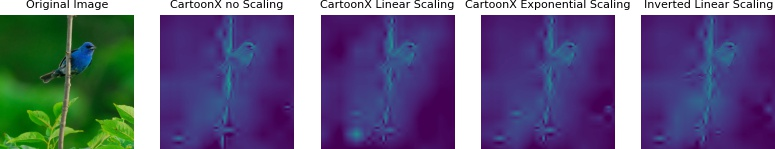
\includegraphics[width=0.7\textwidth]{images/qualitative_ims/obfuscation_examples/indigo.JPEG}
    \caption{Obfuscation experimentation qualitative results for the image of an indigo bird.}
    \label{fig:app-indigo-bird}

\end{figure}

\begin{figure}[H]
    \centering
    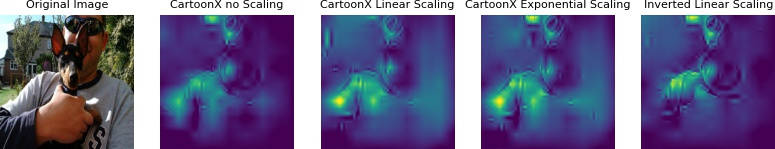
\includegraphics[width=0.7\textwidth]{images/qualitative_ims/obfuscation_examples/terrier.JPEG}
    \caption{Obfuscation experimentation qualitative results for the image of a terrier.}
    \label{fig:app-terrier}

\end{figure}